\documentclass[tikz,border=5pt]{standalone}
\usepackage[T1]{fontenc}
\usepackage{lmodern,amsmath,amssymb}
\usetikzlibrary{arrows.meta,calc,positioning,fit,backgrounds,shapes.geometric,matrix,decorations.pathreplacing,patterns}
\definecolor{ink}{gray}{0.08}
\definecolor{wash}{gray}{0.965}
\definecolor{soft}{gray}{0.45}
\tikzset{box/.style={draw=ink,line width=.65pt,fill=white,align=center,inner sep=4pt,outer sep=0pt,font=\small},flow/.style={draw=ink,line width=.65pt,-{Latex[length=1.8mm,width=1.3mm]},rounded corners=2pt},annotation/.style={font=\scriptsize,text=soft,align=center},groupbox/.style={draw=soft,dashed,line width=.45pt,fill=wash}}
\begin{document}
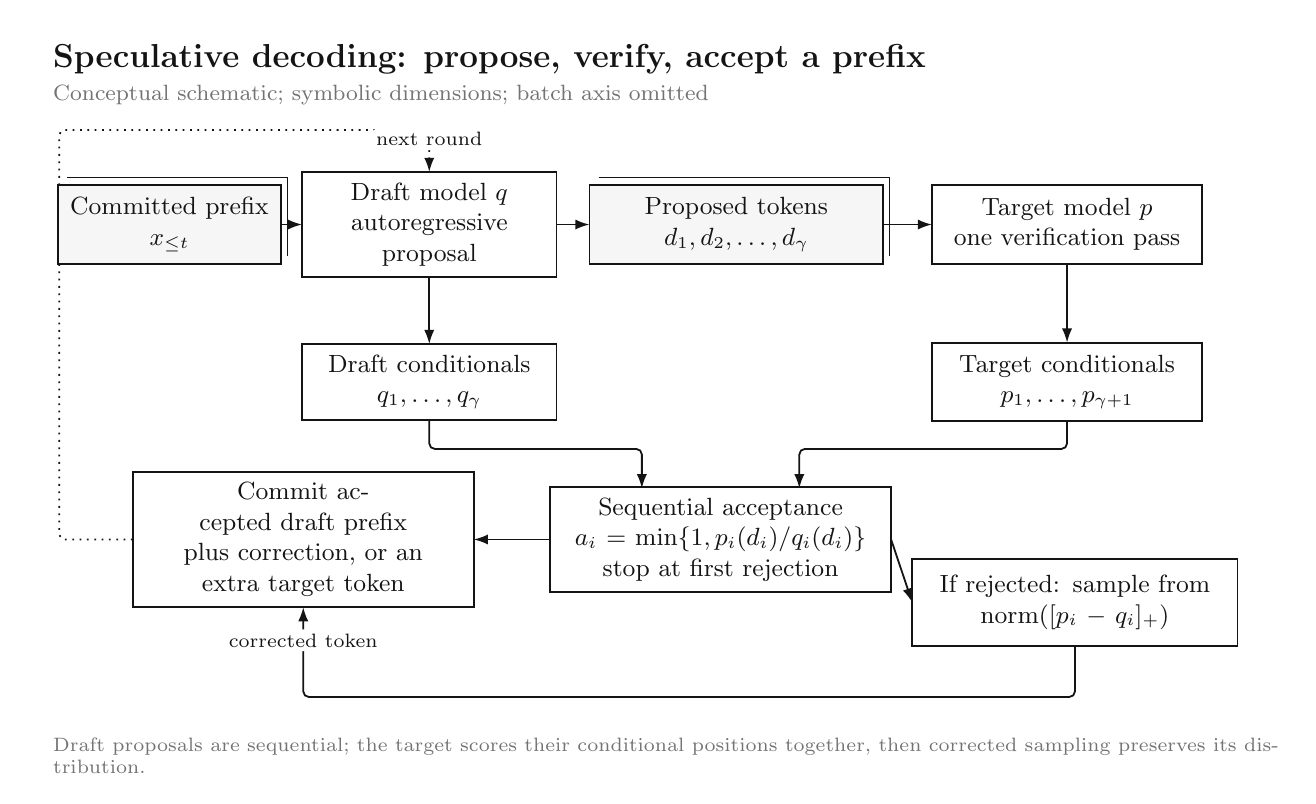
\begin{tikzpicture}[x=1cm,y=-1cm,font=\rmfamily,text=ink]

\path[use as bounding box] (0,0) rectangle (16,9.5);
\node[anchor=west,font=\large\bfseries] at (.2,.4) {Speculative decoding: propose, verify, accept a prefix};
\node[anchor=west,font=\footnotesize,text=soft] at (.2,.85) {Conceptual schematic; symbolic dimensions; batch axis omitted};
\begin{pgfonlayer}{background}
\end{pgfonlayer}
\node[box,fill=wash,minimum width=2.8cm,minimum height=1.0cm,text width=2.55cm] (prefix) at (1.8,2.5) {Committed prefix\\$x_{\leq t}$};
\draw[ink,line width=.4pt] (0.5000000000000001,1.9) -- (3.3000000000000003,1.9) -- (3.3000000000000003,2.9);
\node[box,minimum width=3.2cm,minimum height=1.0cm,text width=2.95cm] (draft) at (5.1,2.5) {Draft model $q$\\autoregressive proposal};
\node[box,fill=wash,minimum width=3.7cm,minimum height=1.0cm,text width=3.45cm] (cand) at (9.0,2.5) {Proposed tokens\\$d_1,d_2,\ldots,d_\gamma$};
\draw[ink,line width=.4pt] (7.25,1.9) -- (10.95,1.9) -- (10.95,2.9);
\node[box,minimum width=3.4cm,minimum height=1.0cm,text width=3.15cm] (target) at (13.2,2.5) {Target model $p$\\one verification pass};
\node[box,minimum width=3.2cm,minimum height=0.9cm,text width=2.95cm] (draftscores) at (5.1,4.5) {Draft conditionals\\$q_1,\ldots,q_\gamma$};
\node[box,minimum width=3.4cm,minimum height=1.0cm,text width=3.15cm] (scores) at (13.2,4.5) {Target conditionals\\$p_1,\ldots,p_{\gamma+1}$};
\node[box,minimum width=4.3cm,minimum height=1.3cm,text width=4.05cm] (accept) at (8.8,6.5) {Sequential acceptance\\$a_i=\min\{1,p_i(d_i)/q_i(d_i)\}$\\stop at first rejection};
\node[box,minimum width=4.1cm,minimum height=1.1cm,text width=3.8499999999999996cm] (correct) at (13.3,7.3) {If rejected: sample from\\$\operatorname{norm}([p_i-q_i]_+)$};
\node[box,minimum width=4.3cm,minimum height=1.3cm,text width=4.05cm] (commit) at (3.5,6.5) {Commit accepted draft prefix\\plus correction, or an extra target token};
\begin{pgfonlayer}{background}
\draw[flow] (prefix.east) -- (draft.west);
\draw[flow] (draft.east) -- (cand.west);
\draw[flow] (cand.east) -- (target.west);
\draw[flow] (target.south) -- (scores.north);
\draw[flow] (draft.south) -- (draftscores.north);
\draw[flow] (accept.west) -- (commit.east);
\draw[flow] (accept.east) -- (correct.west);
\draw[flow] (correct.south) -- (13.3,8.5) -- (3.5,8.5) -- (commit.south) node[midway,above,fill=white,inner sep=1.5pt,font=\scriptsize] {corrected token};
\draw[flow,dotted] (commit.west) -- (0.4,6.5) -- (0.4,1.3) -- (5.1,1.3) -- (draft.north) node[midway,above,fill=white,inner sep=1.5pt,font=\scriptsize] {next round};
\end{pgfonlayer}
\draw[flow] (draftscores.south)--(5.1,5.35)--(7.8,5.35)--(7.8,5.85);
\draw[flow] (scores.south)--(13.2,5.35)--(9.8,5.35)--(9.8,5.85);
\node[anchor=west,align=left,font=\scriptsize,text=soft,text width=15.6cm] at (.2,9.25) {Draft proposals are sequential; the target scores their conditional positions together, then corrected sampling preserves its distribution.};
\end{tikzpicture}
\end{document}
